\usetikzlibrary{calc,intersections}
\tikzset{>=latex} % for LaTeX arrow head
\colorlet{myred}{red!80!black}
\colorlet{myblue}{blue!80!black}
\colorlet{mygreen}{green!60!black}
\colorlet{myorange}{orange!70!red!60!black}
\colorlet{mydarkred}{red!30!black}
\colorlet{mydarkblue}{blue!40!black}
\colorlet{mydarkgreen}{green!30!black}

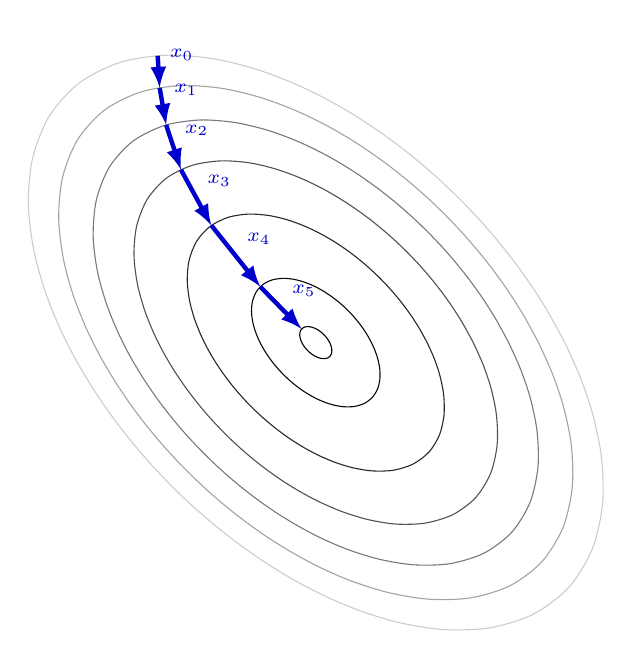
\begin{tikzpicture}[samples=50,smooth]
            %\clip(-4,-1) rectangle (4,4);
            \path[bend left,name path=arrowcurve] (-2,4) to[out=-30,in=-160] (0,0);
            \foreach \y[count=\i] in {20,16,12,8,4,1,0.0625}{
            \pgfmathsetmacro\colper{\y*4} % color percentage variable
                \draw[name path global/.expanded=curve\i,white!\colper!black] plot[domain=0:360] ({cos(\x)*sqrt(\y/(sin(2*\x)+2))},{sin(\x)*sqrt(\y/(sin(2*\x)+2))});
                \draw[name intersections = {of ={curve\i} and arrowcurve}](intersection-1) coordinate (P\i);
                \ifnum\i=1 
                    % do nothing
                \else%
                    \pgfmathtruncatemacro\imin{\i-1}
                    \pgfmathtruncatemacro\iprint{\i-2}
                    \draw[->, myblue, ultra thick] (P\imin) -- (P\i) node[above right,midway] {\scriptsize $x_{\iprint}$}; 
                \fi%
            }     
\end{tikzpicture}